\pdfoutput=1
\documentclass[conference]{IEEEtran}
\usepackage{amsmath,amssymb}
\usepackage{graphicx}
\usepackage{booktabs}
\usepackage{cite}
\usepackage[hidelinks]{hyperref}

% Edit this one line once the repository is public:
\newcommand{\repourl}{\url{https://github.com/MACVXACE/dcd-rls-eeg}}

\begin{document}

\title{Fixed-Point Ridge DCD-RLS Adaptive Filtering for Wearable EEG:\\Hardware Fidelity and Real-Data Comparison Against NLMS}

\author{\IEEEauthorblockN{Varun Bajpai}
\IEEEauthorblockA{Independent Researcher, Kanpur, India\\
varunku3117p@gmail.com}}

\date{}
\maketitle

\begin{abstract}
We implement a fixed-point (Q15/Q30) ridge-regularised leading-element dichotomous coordinate descent recursive least squares (DCD-RLS) adaptive filter requiring 64 multiplies/sample for a single-channel 16-tap filter and 288 multiplies/sample for a 3-axis 48-tap accelerometer filter. In a pre-specified 18-condition semi-synthetic EEGdenoiseNet step-switch benchmark ($f_s = 512$~Hz), integer ridge DCD-RLS improved post-switch relative root-mean-square error (RRMSE) over unregularised integer DCD-RLS (H1: 18/18 cells), unregularised Givens QR-RLS (H4: 18/18 cells), and tuned normalized least-mean-squares (NLMS, $\mu = 0.2$; H3: 17/18 cells), and passed non-inferiority to floating-point ridge least squares (H2) in 8/18 cells. On 23 real accelerometer-referenced PhysioNet motion-artifact EEG recordings ($f_s = 512$~Hz), pre-specified P1 tested whether ridge DCD-RLS exceeded NLMS in $\Delta$SNR over artifact blocks under leave-one-record-out (LORO) tuning. P1 failed: the paired median difference was $-2.116$~dB (95\% CI $[-2.535, -1.971]$~dB, entirely below zero; $p = 4.8\times10^{-7}$; DCD higher on 1/23 records). Clean-EEG preservation (P2) passed ($+0.0145$ RRMSE increase, 95\% CI $[+0.0107, +0.0165] < +0.02$). Exploratory diagnostics showed that the integer filter reproduces float64 ridge RLS within 0.04~dB at $P \ge 9$; ridge RLS gave no advantage over NLMS on these recordings.
\end{abstract}

\begin{IEEEkeywords}
EEG, motion artifact, adaptive filtering, RLS, dichotomous coordinate descent, fixed-point
\end{IEEEkeywords}

\section{Introduction}
Wearable and ambulatory electroencephalography (EEG) recordings are frequently corrupted by non-stationary motion and myogenic artifacts whose spectrum overlaps cortical rhythms. When a correlated noise reference such as a triaxial accelerometer is available, reference-based adaptive noise cancelling can estimate and subtract the coupled interference in real time~\cite{widrow1975}. While normalized least-mean-squares (NLMS) is widely deployed for its $\mathcal{O}(L)$ arithmetic cost, standard recursive least squares (RLS) offers faster convergence across colored inputs at the cost of $\mathcal{O}(L^2)$ matrix-inversion-lemma updates; in our semi-synthetic benchmark, standard float64 RLS diverged at the shortest memory tested. Zakharov \emph{et al.}~\cite{zakharov2008} introduced dichotomous coordinate descent (DCD) RLS solvers that reduce the inner normal-equation solver to bit-shifts and additions; Liu \emph{et al.}~\cite{liu2009} developed FPGA architectures for DCD; and Zakharov and Nascimento~\cite{zakharov2013} proposed DCD-RLS filters with ridge-regression penalties.

Adaptive filtering studies often validate algorithms on semi-synthetic benchmarks such as EEGdenoiseNet~\cite{zhang2021} without testing whether semi-synthetic gains transfer to real multi-sensor motion recordings~\cite{sweeney2012,sweeney2014}. The contributions of this paper are:
\begin{enumerate}
\item A fixed-point (Q15/Q30) implementation of ridge DCD-RLS for multichannel accelerometer references, with a block-shift correlation update, and its evaluation on EEG motion artifact.
\item In a pre-specified 18-cell semi-synthetic path-switch benchmark, four hypotheses (H1--H4) with mixed-to-favourable results: ridge DCD-RLS beat NLMS ($\mu = 0.2$) in 17/18 cells (H3) and passed non-inferiority to floating-point ridge least squares (H2) in 8/18 cells.
\item In a pre-specified evaluation on 23 real PhysioNet motion-artifact EEG recordings, P1 tested whether ridge DCD-RLS exceeded NLMS in $\Delta$SNR over artifact blocks; the 95\% CI lay entirely below zero (median $-2.116$~dB), while clean-EEG non-inferiority (P2) passed.
\item Five exploratory diagnostics (E1--E5) showing that the integer filter reproduces float64 ridge RLS within 0.04~dB at $P \ge 9$ and is not update-limited. Separately, ridge RLS gave no advantage over NLMS on these recordings.
\end{enumerate}

\section{Methods}
``Pre-specified'' means that hypotheses, metrics and pass rules were fixed in code before the evaluation runs reported here. Two deviations are disclosed. The Stage~2 held-out epochs had been used in earlier development rounds, so that test set is not untouched. In Stage~3 the DCD memory grid was extended from $\{5,7,9\}$ to $\{5,7,9,11\}$ under a pre-declared grid-edge rule, after a four-record pilot selected the grid top on all four records; the 23-record run used the extended grid. Line-level provenance for every number is given in the supplementary material.

\subsection{Filter}
Stage~A is a first-order DC blocker, $y[k] = x[k] - x[k-1] + (1-2^{-P_{hp}})\,y[k-1]$ with $P_{hp} = \mathrm{round}(\log_2(f_s/2\pi f_c))$; $f_c = 0.64$~Hz gives $P_{hp} = 7$ at 512~Hz. Stage~B scales and rounds the primary input $d$ and each reference channel to Q15, stacks $L_{ax}$ taps per channel into $\mathbf{u}$, and forms the a-priori error $e = d - (\mathbf{w}^T\mathbf{u} \gg 15)$. With forgetting factor $\lambda = 1-2^{-P}$ applied by shifts, $\mathbf{R}$ and $\mathbf{r}$ are held at Q30:
\begin{align}
\mathbf{R} &\leftarrow \mathbf{R} - (\mathbf{R} \gg P) + \mathbf{u}\mathbf{u}^T,\\
\mathbf{r} &\leftarrow \mathbf{r} - (\mathbf{r} \gg P) + e\,\mathbf{u} - \big((\delta \gg P)\,\mathbf{w}\big) \gg 15,
\end{align}
with $\delta = \gamma\,\mathrm{var}(u)\,2^{P}$ (Q30), a persistent ridge penalty~\cite{zakharov2013}. A leading-element DCD solver~\cite{zakharov2008,liu2009} makes at most $N_u = 4$ coordinate updates per sample over $M_b = 16$ bit levels (amplitude bound $H = 16$), using only shifts, additions and comparisons. With $M$ reference channels, only the $M$ leading columns of $\mathbf{R}$ change per sample; the remaining blocks are shifted, which was bit-identical to the full outer-product update. Stage~2 starts from $\mathbf{R}_0 = \mathrm{var}(u)\,\mathbf{I}$; Stage~3 starts from $\mathbf{R}_0 = \mathbf{0}$.

The single-channel 16-tap filter costs 48 (plain) or 64 (ridge) multiplies and at most 228 or 248 additions/comparisons per sample. The 3-axis 48-tap filter costs 288 multiplies per sample as implemented (48 output, 144 block-shift, 48 $e\mathbf{u}$, 48 leakage). Observed peak signed word lengths in Stage~2 were 35 bits for $\mathbf{R}$, 31--32 bits for $\mathbf{r}$, and 18 bits for $\mathbf{w}$ with ridge versus 22 bits without. Stage~2 scaled each epoch by its own $\max|x| \times 1.05$; Stage~3 scaled each record by the 99.9th percentile of $|x|$ from 2~s to the first artifact onset, $\times 1.05 \times 16$ (headroom), clipping at most 0.061\% of artifact samples.

\begin{figure*}[t]
\centering
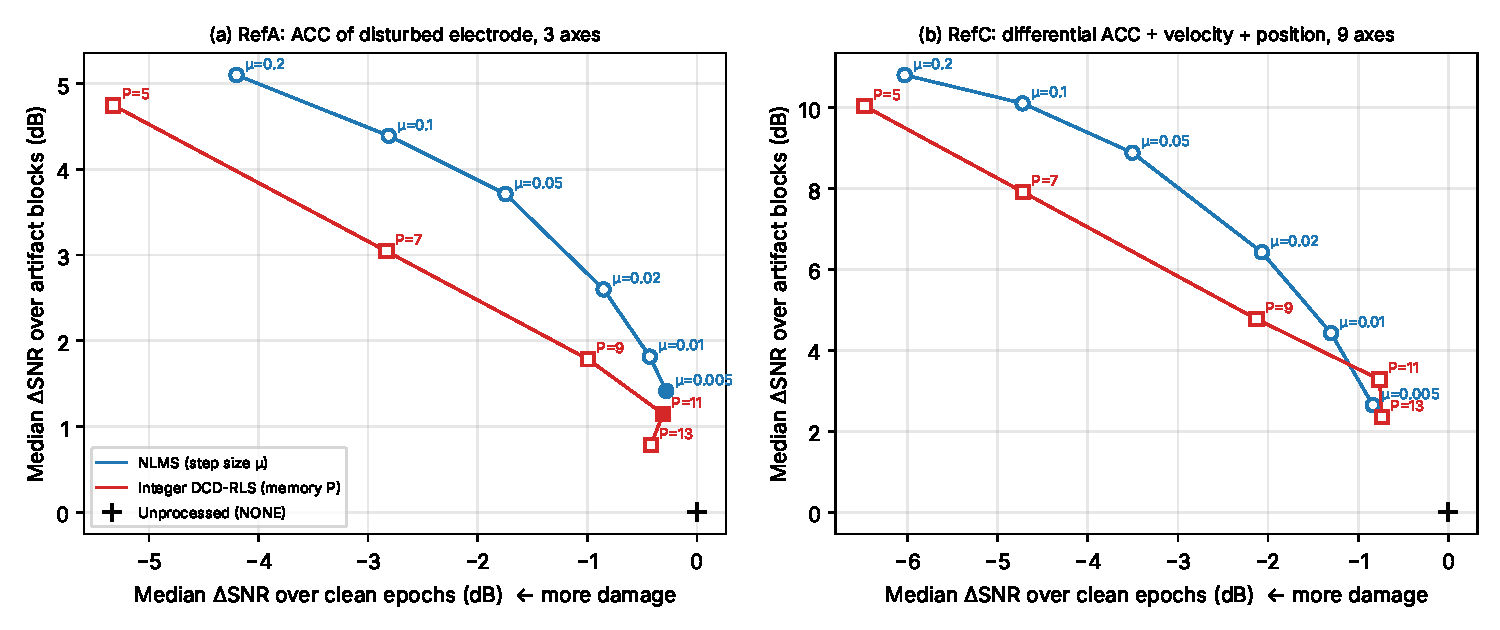
\includegraphics[width=0.92\textwidth]{physionet_tradeoff.pdf}
\caption{Exploratory (E4) removal-versus-preservation trade-off on 23 PhysioNet records: median $\Delta$SNR over clean epochs (x; more negative means more clean-EEG damage) versus median $\Delta$SNR over 60-s artifact blocks (y) for NLMS ($\mu \in \{0.005, \dots, 0.2\}$) and integer ridge DCD-RLS ($P \in \{5, \dots, 13\}$, $N_u = 4$, $\gamma = 0.125$) on (a) RefA (3-axis accelerometer at the disturbed electrode, 48 taps) and (b) RefC (9-axis differential acceleration, velocity and position, 144 taps). Filled markers pass the P2 margin (upper 95\% CI of median clean-epoch RRMSE increase over NONE $< +0.02$): DCD$_\mathrm{RefA}$ at $P = 11$ and NLMS$_\mathrm{RefA}$ at $\mu = 0.005$. Hollow markers fail; the cross marks NONE.}
\label{fig:tradeoff}
\end{figure*}

\subsection{Stage 2: semi-synthetic benchmark}
EEGdenoiseNet~\cite{zhang2021} EEG and EMG epochs were upsampled $2\times$ to 512~Hz (2~s) and z-scored, with disjoint validation (50) and held-out (100) epochs. EMG was passed through a third-order Butterworth 5--100~Hz band-pass for the first second, then $-0.8\times$ a 12--75~Hz band-pass (abrupt path switch), and scaled to input SNR $\in \{-7, -1, +2\}$~dB. The reference was the raw EMG plus white noise at 1, 10 or 31.6\% of its RMS; with $P \in \{4, 5\}$ and $L = 16$ this gives 18 cells. Methods: M1 plain integer DCD-RLS, M2 ridge integer DCD-RLS, M3 float64 ridge exponentially weighted LS, M4 float64 Givens QR-RLS, M5 NLMS, M6 standard float64 RLS. $\gamma \in \{0, 2^{-8}, \dots, 2^{1}\}$ and $\mu \in \{0.05, \dots, 1.0\}$ were tuned on validation epochs (mean of pre- and post-switch RRMSE). On held-out post-switch RRMSE, H1, H3 and H4 (M2 vs M1, M5, M4) pass if the mean paired difference is negative and the two-sided Wilcoxon $p$, Holm-adjusted over 18 cells, is below 0.05; H2 (M2 vs M3) passes if the upper 95\% bootstrap CI (10\,000 resamples) is below $0.02\times\mathrm{mean}(\mathrm{M3})$.

\subsection{Stage 3: real recordings}
The 23 PhysioNet motion-artifact EEG records~\cite{sweeney2014,goldberger2000} were sampled at 2048~Hz; channel EEG1 (FPz) is the reference and motion was applied at EEG2 (FP1h), 20~mm away~\cite{sweeney2012}. Records were decimated $4\times$ to 512~Hz; trigger annotations gave four 60-s artifact intervals per record (240~s). References were RefA, the 3-axis accelerometer at the disturbed electrode (48 taps); RefB, the difference of the two accelerometers; and RefC, RefB plus leaky-integrated velocity and position (144 taps), mean-subtracted over the whole record and hence not strictly causal. $\gamma = 0.125$ was frozen from Stage~2. NLMS normalised each channel by its calibration standard deviation and updated $\mathbf{w} \leftarrow \mathbf{w} + \mu e\mathbf{u}/(\mathbf{u}^T\mathbf{u} + 10^{-4})$. Under leave-one-record-out (LORO) tuning, $P$ (DCD, selected on RefA and reused for RefB/RefC) and $\mu$ were chosen per held-out record to maximise the mean over the other 22 records of $\Delta$SNR$_\mathrm{blocks} + \Delta$SNR$_\mathrm{clean}$, where $\Delta$SNR is the SNR change relative to EEG1~\cite{sweeney2012} over artifact blocks or clean epochs. P1 tested whether DCD on RefA exceeded NLMS on RefA in median $\Delta$SNR over artifact blocks (direction pre-specified; no numeric threshold was coded). P2 passes if the upper 95\% CI of the median clean-epoch RRMSE increase over the unprocessed signal (NONE) is below $+0.02$. CIs are bootstrap intervals of the median (10\,000 resamples) and $p$-values two-sided Wilcoxon; a sensitivity set ($N = 22$) excluded eeg\_20, whose ACC\_x1 channel had 22\% zero-difference samples.

\subsection{Exploratory diagnostics}
Not pre-specified; $p$ unadjusted. E1: $N_u \in \{4, 8, 16\}$. E2: integer DCD versus float64 RLS with the same ridge and with near-zero ridge ($\gamma = 10^{-6}$). E3: $P$ grid extended to 13. E4: trade-off curves over all $\mu$ and $P$ on RefA and RefC, with post-hoc paired Wilcoxon tests. E5: LORO selection of $P$ on RefC itself.

\section{Results}
\subsection{Semi-synthetic benchmark}
Table~\ref{tab:h} summarises the pre-specified tests. At $-7$~dB, the ridge raised pre-switch RRMSE relative to plain DCD-RLS in the 1\% and 10\% noise cells at both $P$ (e.g., $1.198 \to 1.322$), but lowered it at 31.6\% noise, $P = 4$ ($2.029 \to 1.971$). NLMS had the lowest pre-switch RRMSE in four of the six $-7$~dB cells (all $P = 4$ cells and $P = 5$ at 31.6\%); at $P = 5$ with 1\% and 10\% noise, plain DCD-RLS was lowest (1.093, 1.219). Standard float64 RLS diverged at $P = 4$ in all 9 cells (post-switch RRMSE 401--1268) and was stable at $P = 5$.

\begin{table}[t]
\centering
\caption{Pre-specified Stage 2 tests on held-out post-switch RRMSE (18 cells). Range: mean paired difference, M2 minus comparator.}
\label{tab:h}
\begin{tabular}{@{}llcc@{}}
\toprule
H & Comparison & Passed & Range \\
\midrule
H1 & M2 $<$ M1 (plain DCD) & 18/18 & $-0.146$ to $-0.048$ \\
H2 & M2 non-inf.\ M3 (2\%) & 8/18 & $-0.016$ to $+0.066$ \\
H3 & M2 $<$ M5 (NLMS) & 17/18$^{a}$ & $-0.601$ to $-0.020$ \\
H4 & M2 $<$ M4 (QR-RLS) & 18/18 & $-0.338$ to $-0.092$ \\
\bottomrule
\multicolumn{4}{@{}l}{\footnotesize $^{a}$Failing cell: $+2$~dB, 31.6\% noise, $P = 4$ (Holm $p = 0.233$).}
\end{tabular}
\end{table}

\subsection{PhysioNet recordings}
On 23 PhysioNet records ($L_{ax} = 16$, $N_u = 4$, $M_b = 16$, $\gamma = 0.125$; 240~s of artifact in four 60-s intervals per record), pre-specified P1 failed: under LORO (DCD $P = 11$ on 23/23 folds; NLMS $\mu = 0.05$ on 23/23 folds), median $\Delta$SNR$_\mathrm{blocks}$ (DCD$_\mathrm{RefA}-$NLMS$_\mathrm{RefA}$) was $-2.116$~dB ($[-2.535, -1.971]$, $p = 4.8\times10^{-7}$; DCD had the higher $\Delta$SNR on 1/23 records; $N = 22$: $-2.105$~dB $[-2.535, -1.918]$). P2 passed: median clean-RRMSE increase over NONE was $+0.0145$ ($[+0.0107, +0.0165] < +0.02$; $N = 22$: $+0.0146$ $[+0.0107, +0.0170]$), versus $+0.0932$ ($[+0.0667, +0.1053]$) for NLMS ($\mu = 0.05$). In exploratory diagnostics (not pre-specified; $p$ unadjusted), $N_u = 16$ added $+0.011$~dB at $P = 11$ (E1), DCD differed from float64 ridge RLS by $-0.010$~dB ($P = 11$) and $-0.039$~dB ($P = 9$) (E2), and $P = 13$ scored below $P = 11$ ($+0.282$ vs $+1.043$; $P = 11$ on 23/23 folds, an interior optimum, E3). On E4 median curves (Fig.~\ref{fig:tradeoff}), every NLMS$_\mathrm{RefA}$ point lay on the joint frontier and no DCD$_\mathrm{RefA}$ point did; at the two settings that passed P2 (NLMS $\mu = 0.005$, DCD $P = 11$), paired differences were not significant ($p = 0.16$ artifact blocks, $p = 0.111$ clean epochs). RefC LORO (E5) picked $P = 5$ or 7, trailing NLMS$_\mathrm{RefC}$ by $-1.088$~dB on blocks (DCD higher on 6/23 records) and $-1.073$~dB on clean epochs (0/23 records).



\section{Discussion}
The hardware-level contribution of this work stands: on real recordings, the fixed-point DCD implementation reproduces float64 ridge RLS to within 0.04~dB at $P \ge 9$ ($-0.010$~dB at $P = 11$, $-0.039$~dB at $P = 9$) using 288 multiplies per sample for the 48-tap RefA filter, and raising the coordinate-update cap from $N_u = 4$ to 16 alters block $\Delta$SNR by at most $+0.033$~dB at $P \ge 9$, so the integer solver is not bottlenecked by its update budget. By contrast, the algorithmic hypothesis that exponentially weighted ridge RLS improves motion-artifact cancellation over NLMS does not hold on these recordings. At the low-distortion end of the operating curve, where the P2 margin is satisfied on RefA, DCD at $P = 11$ ($+1.15$ / $-0.31$~dB) and NLMS at $\mu = 0.005$ ($+1.42$ / $-0.28$~dB) show no statistically significant difference, which is not evidence of equivalence; on RefA, at higher artifact-removal levels (median values), NLMS achieves greater artifact suppression than any DCD operating point at equal or lower clean-EEG damage. The advantage of integer ridge DCD-RLS over NLMS ($\mu = 0.2$) in the semi-synthetic step-switch benchmark (17/18 cells) did not transfer to real accelerometer-referenced EEG motion artifacts, underscoring that semi-synthetic benchmark advantages do not automatically carry over to real multi-sensor physiological recordings.

\emph{Limitations.} First, all diagnostics (E1--E5) and post-hoc comparisons are exploratory. Second, the ``clean'' signal is an adjacent electrode (EEG1, 20~mm from EEG2) rather than the true cortical signal at EEG2~\cite{sweeney2012}; even unprocessed, the median clean-epoch RRMSE between the two is 0.414, so all metrics are relative to a neighbouring channel. Third, the 0.64~Hz Stage~A filter attenuates 0.5~Hz by 4.17~dB, removing part of the delta band. Fourth, NLMS and DCD were tuned with the same composite LORO objective; on RefC (E5) it selected $P = 5$ or 7, both with median clean-epoch $\Delta$SNR below $-4.7$~dB. Fifth, the real-data evaluation uses a single dataset of 23 recordings. Sixth, the semi-synthetic benchmark compared against NLMS at a single tuned step size ($\mu = 0.2$) rather than a full trade-off curve. Seventh, Stage~2 used non-causal per-epoch scaling; causal validation-set scaling changed held-out post-switch RRMSE by at most $+0.017$. Eighth, RefC is not strictly causal (whole-record mean removal).

\section{Conclusion}
We presented a fixed-point (Q15/Q30) ridge DCD-RLS adaptive filter costing 64 multiplies/sample for a 16-tap single-channel filter and 288 for a 48-tap three-axis filter. On 23 real PhysioNet motion-artifact EEG records it reproduced float64 ridge RLS within 0.04~dB at $P \ge 9$ and passed clean-EEG preservation (P2), but P1 failed: median $\Delta$SNR versus NLMS was $-2.116$~dB, 95\% CI entirely below zero. The semi-synthetic advantage (17/18 cells) did not transfer.

\section*{Data and Code Availability}
All scripts, output logs and the per-number verification tables are archived at \repourl. Data: EEGdenoiseNet~\cite{zhang2021}; PhysioNet~\cite{sweeney2014}.

\section*{Acknowledgments}
The author conceived the study, designed the pre-specified benchmarks, ran the PhysioNet evaluations, and verified every reported result against the raw output logs. Large language models (Anthropic's Claude and Google's Gemini) were used as assistive tools for software implementation, semi-synthetic benchmark execution, code auditing, and manuscript drafting.

\IEEEtriggeratref{3}
\begin{thebibliography}{8}
\bibitem{widrow1975} B. Widrow \emph{et al.}, ``Adaptive noise cancelling: Principles and applications,'' \emph{Proc. IEEE}, vol.~63, no.~12, pp.~1692--1716, Dec. 1975, doi:10.1109/PROC.1975.10036.
\bibitem{zakharov2008} Y. V. Zakharov, G. P. White, and J. Liu, ``Low-complexity RLS algorithms using dichotomous coordinate descent iterations,'' \emph{IEEE Trans. Signal Process.}, vol.~56, no.~7, pp.~3150--3161, Jul. 2008, doi:10.1109/TSP.2008.917874.
\bibitem{liu2009} J. Liu, Y. V. Zakharov, and B. Weaver, ``Architecture and FPGA design of dichotomous coordinate descent algorithms,'' \emph{IEEE Trans. Circuits Syst. I, Reg. Papers}, vol.~56, no.~11, pp.~2425--2438, Nov. 2009, doi:10.1109/TCSI.2009.2015725.
\bibitem{zakharov2013} Y. V. Zakharov and V. H. Nascimento, ``DCD-RLS adaptive filters with penalties for sparse identification,'' \emph{IEEE Trans. Signal Process.}, vol.~61, no.~12, pp.~3198--3213, Jun. 2013, doi:10.1109/TSP.2013.2258340.
\bibitem{zhang2021} H. Zhang, M. Zhao, C. Wei, D. Mantini, Z. Li, and Q. Liu, ``EEGdenoiseNet: a benchmark dataset for deep learning solutions of EEG denoising,'' \emph{J. Neural Eng.}, vol.~18, no.~5, p.~056057, 2021, doi:10.1088/1741-2552/ac2bf8.
\bibitem{sweeney2012} K. T. Sweeney, H. Ayaz, T. E. Ward, M. Izzetoglu, S. F. McLoone, and B. Onaral, ``A methodology for validating artifact removal techniques for physiological signals,'' \emph{IEEE Trans. Inf. Technol. Biomed.}, vol.~16, no.~5, pp.~918--926, Sep. 2012, doi:10.1109/TITB.2012.2207400.
\bibitem{sweeney2014} K. Sweeney \emph{et al.}, ``Motion artifact contaminated fNIRS and EEG data (version 1.0.0),'' PhysioNet, 2014, doi:10.13026/C2988P.
\bibitem{goldberger2000} A. L. Goldberger \emph{et al.}, ``PhysioBank, PhysioToolkit, and PhysioNet: Components of a new research resource for complex physiologic signals,'' \emph{Circulation}, vol.~101, no.~23, pp.~e215--e220, 2000, doi:10.1161/01.CIR.101.23.e215.
\end{thebibliography}

\end{document}
